\documentclass[11pt]{beamer}
\usepackage[utf8]{inputenc}
\usepackage[francais]{babel}
\usepackage[T1]{fontenc}
\usepackage{graphicx}

\usetheme{CambridgeUS}

\author{Cortier — Lazare — Boulmier}
\institute[]{UTBM}
\title{Soutenance de projet d'IA41}
\subtitle{Sujet : Force 3}
\logo{\includegraphics[width=0.12\textwidth]{logo}}

\date{23 juin 2017}

\subject{Force 3}

\graphicspath{{../report/fig/}}

\beamertemplatenavigationsymbolsempty{} % remove navigation symbols.

\begin{document}

\begin{frame}
    \titlepage{}
\end{frame}

\begin{frame}{Table des matières}
    \tableofcontents
\end{frame}

\section{Structures de données}

\begin{frame}
    \begin{block}{lorem ipsum}
            \begin{itemize}
                \item Case
                \item Plateau de jeu
                \item État du jeu
            \end{itemize}
    \end{block}
\end{frame}

\section{Algorithme du néga-max}

\begin{frame}
    Min-max :
    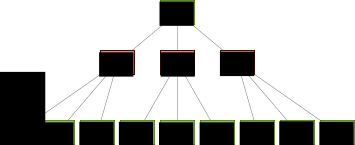
\includegraphics[width=\linewidth]{minmax}
\end{frame}

\begin{frame}
    Néga-max :
    \includegraphics[width=\linewidth]{negamax}
\end{frame}

\begin{frame}
    Élagage alpha-béta :
    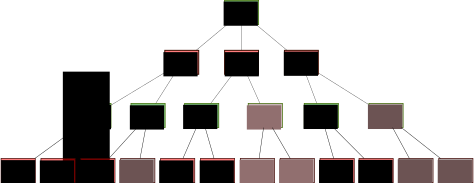
\includegraphics[width=\linewidth]{negamax-alphabeta}
\end{frame}

\section{Heuristiques}

\begin{frame}
    \emph{Facile (win-lose)} :
    Pour un plateau donné, elle renvoie la valeur maximum si l'I.A. a gagné, la valeur minimum si
    l'I.A. a perdu, et 0 si aucun joueur n'a gagné.
\end{frame}

\begin{frame}
    \emph{Normale} :
    \includegraphics[width=\textwidth]{Heuristic_Normal}{}
\end{frame}

\begin{frame}
    \emph{Difficile} :
    \includegraphics[width=\textwidth]{Heuristic_Hard}{}
\end{frame}

\begin{frame}
    \emph{Légendaire} :
    \includegraphics[width=\textwidth]{Heuristic_Legendary}{}
\end{frame}

\section{Résultats}

\begin{frame}
    \begin{itemize}
        \item Nous avons découvert que le premier joueur a toujours moyen de gagner entre 4 et 6 coups
            (on a au début cru à une anomalie de l'algorithme nega-max).
        \item Il est aussi possible de tomber dans des cycles (ou états stables) où aucun joueur ne peut gagner.
        \item Nous avons pu classer les heuristiques selon le nombres de parties gagnées contre telle ou telle heuristiques à
            telle ou telle profondeur en faisant un mini tournoi d'IA\@. C'est là qu'on leur a donné leur nom « facile », « normal », …
        \item Il est aussi clair que l'IA est meilleure que le joueur à partir d'une certaine profondeur en particulier pour les
            heuristiques « difficile » et « légendaire ».
    \end{itemize}
\end{frame}

\end{document}

